In this chapter we show how to implement languages in Metacasanova. The first language that we implement is a small imperative language called C-{}-. Although tiny, this language contains many common features typical of imperative languages such as control structures, program states, variable scoping, and type annotations. We then proceed to re-implement the semantics of Casanova, a DSL for game development, in Metacasanova, similar to the work shown also in \cite{DiGiacomo2017}. Finally, we evaluate the length of the language implementation in Metacasanova against a hard-coded implementation of the same language in a general-purpose programming language, and the runtime performance of programs written in the meta-compiled version against Python.

\section{The C-{}- language}
In this section we present the implementation of a small imperative language called C-{}-. Note that, although the name might suggest this, we do not claim any resemblance with the C programming language, as it lacks several features such as pointer arithmetic, arrays, and functions.

C-{}- allows the use of four built-in values: integers, strings, boolean values, and floating-point numbers in double precision. The language provides three kinds of control structures: if-then-else, while-do, and for loops with the same semantics as usual for imperative languages. The language supports variable scoping and shadowing.

The memory is represented using a dictionary that pairs variable names with their value. In what follows we omit the details of the lookup of entries in the dictionary for brevity. Suffice to say that the meta-program makes use of the \texttt{ImmutableDictionary} data structure available in .NET. Also note that C-{}- defines scopes for variables, so that if a variable is declared inside the scope of a code block in a control structure, that is usable only within the scope itself.

The core of the meta-program is made of the evaluation of both expressions and statements. We proceed below to present the details of both kinds of evaluations.

\subsection{Expression Semantics}
\label{subsec:ch_mcnv_languages_expression_semantics}
As explained above C-{}- supports boolean, string, integer, and floating-point values. These are represented through the following meta-data structures in the meta-program.

\begin{lstlisting}
Data "$i" -> <<int>> : Value Priority 300
Data "$d" -> <<double>> : Value Priority 300
Data "$s" -> <<string>> : Value Priority 300
Data "$b" -> <<bool>> : Value Priority 300
\end{lstlisting}

\noindent
Note that we are using the .NET data types to represent the actual values stored in the meta-data structures. We also define the following subtype, since values are atomic cases of expressions and can be used as such:

\begin{lstlisting}
Value is Expr
\end{lstlisting}

\noindent
Expressions can also contain variables, thus we need a meta-data structure to represent them as well.

\begin{lstlisting}
Data "$" -> <<string>> : Id Priority 300
\end{lstlisting}

\noindent
Variables can be used as atomic expressions as well, so we need an additional subtype

\begin{lstlisting}
Id is Expr
\end{lstlisting}

\noindent
We now define a data structure to represent the state of the program. The state is simply a map where the key is a variable name and the stored element a valid value in C-{}-. In the declaration we will define the meta-type \texttt{SymbolTable}, and from now on we will refer use the term ``symbol table'' as a synonym of ``state''.

\begin{lstlisting}
Data "$m" << ImmutableDictionary<Id, Value> >> : SymbolTable 
\end{lstlisting}

\noindent
Since we want to allow variable scoping, the state of the program is not represented by a single map, but by a list of maps. Each time the program enters a different scope context, an empty map is added to this list, and removed when the program exits the scope. This process will be further explained below. We define a meta-data structure to represent this list of states (note that the operator for the construction of the list is infix).

\begin{lstlisting}
Data SymbolTable -> "::" -> TableList : TableList
Data "[]" -> TableList
\end{lstlisting}

\noindent
We can now proceed to define a meta-data structure to represent the operations for expressions. First we define the arithmetic operators in the language:

\begin{lstlisting}
Data Expr -> "+" -> Expr : Expr
Data Expr -> "-" -> Expr : Expr
Data Expr -> "*" -> Expr : Expr
Data Expr -> "/" -> Expr : Expr
\end{lstlisting}

\noindent
then we can define operators for boolean expressions:
\begin{lstlisting}
Data Expr -> "&&" -> Expr : Expr
Data Expr -> "||" -> Expr : Expr
Data "!" -> Expr : Expr
\end{lstlisting}

\noindent
and finally comparison operators:
\begin{lstlisting}
Data Expr -> "equals" -> Expr : Expr
Data Expr -> "neq" -> Expr: Expr
Data Expr -> "ls" -> Expr : Expr
Data Expr -> "leq" -> Expr : Expr
Data Expr -> "grt" -> Expr : Expr
Data Expr -> "geq" -> Expr : Expr
\end{lstlisting}

We now have to define the function that evaluates an expression through rules in the program. This function takes as input the list of symbol tables (needed to read possible variables), an expression, and returns the value after computing the expression.

\begin{lstlisting}
Func "evalExpr" -> TableList -> Expr : Value
\end{lstlisting}

\noindent
Now we have to proceed to define the rules to compute the actual evaluation of an expression. Clearly the base cases of the evaluation are the atomic values, where we immediately return the value itself.

\begin{lstlisting}
-----------------------------
evalExpr tables ($i v) -> ($i v)

-----------------------------
evalExpr tables ($d v) -> ($d v)

-----------------------------
evalExpr tables ($s v) -> ($s v)

-----------------------------
evalExpr tables ($b v) -> ($b v)
\end{lstlisting}

Evaluating variables is more complex: we have to look at the table currently in the head of the list of tables (which is the one relative to the current scope). If we do not find the required variable we have to recursively look it up in the tail of the list, since we could have an arbitrary number of nested scopes. When the variable is found we return its value. This behaviour is implemented by the following code:

\begin{lstlisting}
symbols contains ($name) -> Yes
symbols lookup ($name) -> val
-------------------------------------------
evalExpr (symbols :: tables) ($name) -> val

symbols contains ($name) -> No
evalExpr tables ($name) -> val
-------------------------------------------
evalExpr (symbols :: tables) ($name) -> val

\end{lstlisting}

We proceed now to define the evaluation of arithmetic operators. We show only the example of the sum for brevity, the other rules differ only in the operator. Evaluating the arithmetic expression requires to recursively call \texttt{evalExpr} on the right and left argument. These recursive calls will eventually return two values that are the result of the two evaluations. After we obtain these values, we can compute their sum and return it as result.

\begin{lstlisting}
evalExpr tables expr1 -> ($i val1)
evalExpr tables expr2 -> ($i val2)
<<val1 + val2>> -> v
---------------------------------------
evalExpr tables expr1 + expr2 -> ($i v)
\end{lstlisting}

\noindent
Note that we have used .NET external code in the third premise to compute the result of the arithmetic operation. Evaluating arithmetic operations involving floating-point expressions can be done in an analogous way, except in the premises we expect to have the meta-data structure for floating-point values as result of \texttt{evalExpr}:

\begin{lstlisting}
evalExpr tables expr1 -> ($d val1)
evalExpr tables expr2 -> ($d val2)
<<val1 + val2>> -> v
---------------------------------------
evalExpr tables expr1 + expr2 -> ($d v)
\end{lstlisting}

\noindent
The same can be said for the string concatenation.
The evaluation of boolean expression is analogous: we show again only the evaluation for AND as the other rules are analogous:

\begin{lstlisting}
evalExpr tables expr1 -> ($b val1)
evalExpr tables expr2 -> ($b val2)
<<val1 && val2>> -> b
----------------------------------
evalExpr tables expr1 && expr2 -> b
\end{lstlisting}

\noindent
Again we rely on external code to compute the actual boolean value.
As for the comparison operators, we can use a clause in the premise to avoid using external code in the following way:

\begin{lstlisting}
evalEpxr tables expr1 -> val1
evalExpr tables expr2 -> val2
val1 == val2
-----------------------------------------------
evalExpr tables (expr1 equals expr2) -> $b true

evalEpxr tables expr1 -> val1
evalExpr tables expr2 -> val2
val1 != val2
------------------------------------------------
evalExpr tables (expr1 equals expr2) -> $b false
\end{lstlisting}

\noindent
The first rule checks that the values computed by evaluating the left and right argument of the equality comparison are the same. If this happens then the rule returns a meta-data structure containing the boolean representation of \texttt{true}. Otherwise the first rule fails and the second one is executed. This one will return a boolean representation of \texttt{false} when the values are different.

For inequality operators we must rely on external code for the computation is Metacasanova only allows equality comparisons in clauses:

\begin{lstlisting}
evalExpr tables expr1 -> ($i val1)
evalExpr tables expr2 -> ($i val2)
<< val1 < val2 >> -> boolResult
---------------------------------------------------
evalExpr tables (expr1 ls expr2) -> ($b boolResult)
\end{lstlisting}

\noindent
The evaluation of the other comparison operators is implemented through analogous rules, which differ only in the operators.

\subsection{Statement Semantics}
\label{subsec:ch_mcnv_languages_statement_semantics}

Statement evaluation requires the definition of a different function, \texttt{eval}, that processes each statement and returns the result of the statement evaluation and the updated state. Note that, even if the evaluation of statements does not always change the state, in general we have to assume that this will happen.

The function \texttt{eval} takes as input a statement to process and the current state (list of symbol tables), and returns the updated list of symbol tables

\begin{lstlisting}
Func "eval" -> TableList -> Stmt : TableList
\end{lstlisting}

We now proceed to define the meta-data structures necessary to represent the statements of the language: C-{}- supports (\textit{i}) variable declarations, (\textit{ii}) variable assignment, (\textit{iii}) if-then-else, (\textit{iv}) while loops, and (\textit{v}) for loops.

Variable declarations follow the same structure of standard C, that is a type name followed by an identifier. Thus, the corresponding meta-data structure can be defined as:

\begin{lstlisting}
"variable" -> Type -> Id : Stmt
\end{lstlisting}

\noindent
Analogously, variable assignment follows the C convention and uses the \texttt{=} symbol.

\begin{lstlisting}
Id -> "=" -> Expr : Stmt
\end{lstlisting}

The control structure if-then-else does not follow the standard C representation, rather we use the keywords \texttt{then} and \texttt{else} to delimit its code blocks. Note that nothing prevents us from implementing the conventional C syntax, but we prefer this ``lightweight'' representation. The keywords \texttt{then} and \texttt{else} are meta-data structures that take no arguments and do not have any functional utility other than syntactical mark-ups.

\begin{lstlisting}
Data "then" : Then
Data "else" : Else
Data "if" -> Expr -> Then -> Stmt -> Else -> Stmt : Stmt
\end{lstlisting}

Analogously we can define the meta-data structure for \texttt{While} and \texttt{For}

\begin{lstlisting}
Data "do" : Do
Data "while" -> Expr -> Do -> Stmt : Stmt
Data "for" -> Expr -> Expr -> Epxr -> Do -> Stmt : Stmt
\end{lstlisting}

\noindent
Up to this point we are able to define single statements in the language, but we need a way to concatenate a sequence of statements to form code blocks, in the fashion of C. This is done by introducing an additional meta-data structure, which is the ";" symbol. For convenience, we also introduce a \texttt{nop} statement, which does not do anything, but it will be useful to express the semantics of statements evaluation.

\begin{lstlisting}
Data Stmt -> ";" -> StmtList : StmtList
Data "nop" -> :Stmt

StmtList is Stmt

\end{lstlisting}

We now proceed to define the semantics of statement evaluation.

\subsubsection{Evaluating a Sequence of Statements}
The evaluation of a sequence of statements require to evaluate the first statement in a sequence and then recursively evaluate the rest of the sequence. The recursive evaluation returns the final program state. The base case of the recursion is met when the sequence contains only \texttt{nop}. In this case we terminate the evaluation and return the unchanged program state.

\begin{lstlisting}
--------------------------
eval tables nop -> tables

eval tables a -> tables'
eval table' b -> res
---------------------------
eval tables (a;b) -> res
\end{lstlisting}

\subsubsection{Variable Declarations and Assignments}
Evaluating a variable declaration simply adds the variable to the symbol table of the current scope. Note that we allow variable shadowing, so it is possible to redefine the same symbol in different scopes.

\begin{lstlisting}
symbols defineVariable id -> symbols'
-------------------------------------
eval (symbols nextTable tables) (variable t id) -> symbols' nextTable tables
\end{lstlisting}

\noindent
This rule is executed whenever the processed statement matches the structure of a variable declaration statement. The premise adds the symbol to the symbol table of the current scope (we omit the details for brevity), and returns an updated symbol table. The list of symbol 
tables is rebuilt to include the updated table and returned as result.

Variable assignment is more complex, since the variable we are trying to use might not be in the symbol table of the current scope. We must then define two lookups functions, that behave differently depending on whether the variable is in the symbol table in the head of the symbol table list or not. We declare the function \texttt{updateTable} that performs this lookup and updates the table list accordingly. 

\begin{lstlisting}
Func "updateTables" -> TableList -> TableList -> Id -> Expr : EvaluationResult
\end{lstlisting}

\noindent
In the case that the variable is in the symbol table in the head of the list of tables we have the following rule:

\begin{lstlisting}
symbols contains id -> Yes
evalExpr vars expr -> val
symbols add id val -> symbols'
-------------------------------
updateTables vars (symbols :: tables) id expr -> symbols' :: tables
\end{lstlisting}

\noindent
The first premise checks if the symbol is contained in the table in the head of the list. If the answer is \texttt{Yes} (a meta-data structure returned by the function \texttt{contains}, not described here again for brevity), then the second premise proceeds to evaluate the expression in the right hand-side of the assignment. The third premise adds the value obtained as result of the second premise to the current symbol table and returns the modified table. The new table is then placed in the head of the table list and the whole list is returned. Note that, at this point, all the tables in the list remain unchanged except the one that was in the head. Note that \texttt{updateTables} carries two copies of the list of tables. One of them is passed to \texttt{eval} because the right-hand side of the assignment might contain other variables. The process of looking up the left hand-side variable pops symbol tables from the head of list (see next rule) but the original list of tables is necessary when assigning the values of variables located in inner scopes. For instance, consider the following program in C-{}-:

\begin{lstlisting}[caption = C-{}- sample program, label = code:ch_mcnv_languages_c--_sample_program]
int x;
...
if (x > 0) then
	int y;
	y = 4
	x = y;
else
  x = x - 1;	
\end{lstlisting}

\noindent
assume that before the if-then-else $x > 0$. The program will enter the \texttt{then} block and declare \texttt{y}. In the current state we have to symbol tables, one for the scope of the \texttt{if-then-else} and one for the outer scope. When assigning \texttt{y} to \texttt{x} the symbol table tries to look up \texttt{x} in the table of the current scope and fails. This will pop the head of the list of tables (which is the table of \texttt{if-then-else}) and recursively look in the tail. During the second attempt \texttt{x} is retrieved but now we do not have the symbol table where \texttt{y} is defined anymore to evaluate the right hand-side. We thus need the original list of tables to be able to retrieve \texttt{y}. In general, if we call \texttt{$d_l$} the depth of scoping of the left hand-side and $d_r$ the depth of scoping of the right hand-side, the process pops the table of the right hand-side whenever $d_l > d_r$ and this is when we need the original list of tables to retrieve the value of the right hand-side.

If the variable is not contained in the head of the list, i.e. it has not been declared in the current scope, we have the following rule:

\begin{lstlisting}
symbols contains id -> No
updateTables vars tables id expr -> tables'
----------------------------------------------
updateTables vars (symbols :: tables) id expr -> symbols :: tables'
\end{lstlisting}

The first premise tries to lookup the variable in the symbol table of the current scope and does not find it. Thus we recursively call \texttt{updateTables} with the tail of the list. The recursive call will eventually find the variable in one of the symbol tables associated with outer scopes. This process will produce an updated list of tables that is returned as a new tail for the current list.

At this point, the rule for the evaluation of the variable assignment simply class the \texttt{updateTables} function in its premise:

\begin{lstlisting}
updateTables tables tables id expr -> res
----------------------------------------
eval tables (id = expr) -> res
\end{lstlisting}

\subsubsection{Conditionals}

Evaluating \texttt{if-then-else} requires two rules, depending on the result of the evaluation of its condition. The following rule implements the semantics when the condition is false:

\begin{lstlisting}
evalExpr tables condition -> $b true
emptyDictionary -> table
eval (table :: tables) thenBlock -> table' :: tables''
-------------------------------------------
eval tables (if condition then thenBlock else elseBlock) -> tables''
\end{lstlisting}

The first premise evaluates the condition of the control structures and succeeds if the result is a meta-data structure containing the boolean value \texttt{true}. The second premise uses an utility function to initialize an empty symbol table. This is required to define a new table for the scope of the conditional. The third premise evaluates the statements contained in the then block after pushing the symbol table for the current scope in the list of symbol tables. This process will eventually produce a new list of symbol tables. The result returns only the tail of this list, since when we exit the scope of the conditional we must pop its symbol tables.

For instance, consider again the program in Listing \ref{code:ch_mcnv_languages_c--_sample_program} and again assume that $x > 0$. After executing the then block, the state of the program is made of the symbol tables shown in Table \ref{tab:ch_mcnv_languages_tables_ifthenelse}. After exiting the then block, variable \texttt{y} exits the scope, thus we have to pop the symbol table for the current scope. However, the symbol table of the outer scope has been changed because \texttt{x} got the value of \texttt{y}. Thus the evaluation returns the list containing this updated table. In general, the process should consider that an arbitrary number of symbol tables for each outer scope has been changed, thus we return this updated list.

\begin{table}
	\centering
	\begin{tabular}{|l|l|}
		\hline
		\textbf{Variable} & \textbf{Value} \\
		\hline
		x & undefined\\
		\hline
	\end{tabular}\\
	\vspace{0.2cm}
	\begin{tabular}{|l|l|}
		\hline
		\textbf{Variable} & \textbf{Value} \\
		\hline
		y & 4\\
		\hline
	\end{tabular}
	\begin{tabular}{|l|l|}
		\hline
		\textbf{Variable} & \textbf{Value} \\
		\hline
		x & 4\\
		\hline
	\end{tabular}
	\caption{Symbol table at the beginning and after the execution of the program in Listing \ref{code:ch_mcnv_languages_c--_sample_program} with $x > 0$}
	\label{tab:ch_mcnv_languages_tables_ifthenelse}
\end{table}

The rule that evaluates conditionals when the condition is false is analogous, except this time we evaluate the else block:

\begin{lstlisting}
evalExpr tables condition -> $b false
emptyDictionary -> table
eval (table :: tables) elseBlock -> table' :: tables''
--------------------------------------------
eval tables (if condition then thenBlock else elseBlock) -> tables''
\end{lstlisting}

\subsubsection{While Loops}
\label{subsec:ch_mcnv_languages_cmm_loops}
Evaluating the while loops require to check its condition first. When the condition is false we simply skip the loop without changing the state. The rule to implement this behaviour is thus straightforward:

\begin{lstlisting}
evalExpr tables condition -> $b false
--------------------------------------------
eval tables (while condition do block) -> tables
\end{lstlisting}

\noindent
The semantics when the condition is true is more complex:

\begin{lstlisting}
evalExpr tables condition -> $b true
emptyDictionary -> table
eval (table :: tables) block -> table' :: tables''
eval tables'' (while condition do block) -> res
---------------------------------------------------
eval tables (while condition do block) -> res
\end{lstlisting}

\noindent
The first premise succeeds when the evaluation of the condition returns a true boolean value in C-{}-. Analogously to what we did for conditionals, we initialize an empty symbol table for the current scope and we push it into the list of symbol tables. We then evaluate the body of the loop. This process will, in general, produce an updated list of symbol tables. Again we pop the symbol table for the current scope because we are exiting the loop. We then evaluate again the whole loop to test its condition again.

\subsubsection{For Loops}
For loops follow the C convention and are made of four parts: (\textit{i}) an initialization, (\textit{ii}) a condition (\textit{ii}), (\textit{iii}) a step, and (\textit{iv}) a block of code. The initialization is evaluated once before entering the loop, the condition is tested before each iteration of the loop, and the step is evaluated at the end of each iteration. In order to implement this behaviour we make use of an additional support function called \texttt{loopFor}:

\begin{lstlisting}
Func "loopFor" -> TableList -> Expr -> Stmt -> Stmt : TableList
\end{lstlisting}

\noindent
The evaluation of the \texttt{for-loop} evaluates the initialization in its premise. It then calls \texttt{loopFor} after the initialization has been evaluated. Again the initialization might define additional variables that enter the scope of the loop, so the updated table of the current scope is pushed into the list of symbol tables. Note that possible variables defined in the initialization part of the loop might be used after the loop itself, according to the semantics of C, so we have to insert them into the symbol table of the current scope and not the one of the loop itself.

\begin{lstlisting}
eval tables init => tables'
loopFor tables' condition step block => res
-------------------------------------------------------
eval tables (for init condition step do block) => res
\end{lstlisting}

The rules for \texttt{loopFor} are two, since we must consider the case when the condition is false and the one where it is true. When the condition is false the loop is completely skipped, thus we simply return the current state without any changes, in the same fashion of the \texttt{while-loop}:

\begin{lstlisting}
evalExpr tables condition -> $b false
--------------------------------------
loopFor tables condition step block -> tables
\end{lstlisting}

\noindent
When the condition is true, we create as usual a symbol table for the scope of the loop and we push it into the list of symbol tables. The third premise evaluates the block of the loop returning an updated list of tables. As usual we pop the table of the scope of the loop and we evaluate the step. This again might change the list of symbol tables. We then run again the loop with the updated list of tables.

\begin{lstlisting}
evalExpr tables condition -> $b true
emptyDictionary -> table
eval (table :: tables) block -> table' :: tables''
eval tables'' step -> tables3
loopFor tables3 condition step expr -> res 
-------------------------------------------------
loopFor tables condition step block -> res
\end{lstlisting}

\subsection{Type Checker}
\label{subsec:ch_mcnv_languages_type_checking}
Type checking can be performed by using a representation of the type system of C-{}- in terms of rules, in the same fashion of the semantics. In this section we explain the details of how each language construct is type-checked according to its type rule. We begin by defining an alternative version of the symbol table defined in Section \ref{subsec:ch_mcnv_languages_expression_semantics} that contains a mapping between variable names and types:

\begin{lstlisting}
Data "$m" << ImmutableDictionary<Id, Type> >> : TypeTable 
\end{lstlisting}

\noindent
and a constructor for the meta-data representing a sequence of type tables.

\begin{lstlisting}
Data TypeTable -> "::" -> TypeTableList : TypeTableList
Data "[]" : TypeTable
\end{lstlisting}

\noindent
We now start by defining the meta-data structures for the types in C-{}-:

\begin{lstlisting}
Data "t_int" : Type
Data "t_double" : Type
Data "t_string" : Type
Data "t_bool" : Type
Data "t_unit" : Type
\end{lstlisting}

\noindent
We also defined a special meta-data representing a type error to correctly report errors if the program contains invalid types:

\begin{lstlisting}
Data "error" -> <<string>> : Type
\end{lstlisting}

\subsubsection{Typing expressions}

We now proceed to define the type rules for expressions. We initially need to define a function to use in the conclusion of a type rule that is able to evaluate type of an expression:

\begin{lstlisting}
Func "typeExpr" -> TypeTableList -> Expr : Type
\end{lstlisting}

The axioms of expression typing are those that return the type of a literal. In this case the rule immediately returns the type associated to the specific literal.

\begin{lstlisting}
-----------------------------
typeExpr tables ($i v) -> t_int

-----------------------------
typeExpr tables ($d v) -> t_double

-----------------------------
typeExpr tables ($s v) -> t_string

-----------------------------
typeExpr tables ($b v) -> t_bool
\end{lstlisting}

\noindent
Type checking variables require to perform a lookup for the variable name in the list of type tables that we carry along during the typing process. The variable could be in the table associated with the current scope or in the table of an outer scope. Therefore, we start by first looking in the table of the current scope, and if we do not find the variable we recursively look it up in the subsequent table. If we traverse the whole list of tables without finding the variable, then it means that the program contains an undefined variable and an appropriate error notifying the problem should be returned.

\begin{lstlisting}
-------------------------------------
typeExpr [] ($ name) -> error <<"Undefined variable:" + name>>

types contains ($ name) -> Yes
types lookup ($ name) -> varType
------------------------------------------------
typeExpr (types :: tables) ($ name) -> varType

types contains ($ name) -> No
typeExpr tables ($ name) -> error msg
------------------------------------------
typeExpr (types :: tables) ($ name) -> error msg 

types contains ($ name) -> No
typeExpr tables ($ name) -> varType
------------------------------------------
typeExpr (types :: tables) ($ name) -> varType 
\end{lstlisting}

Note that we had to include a rule in whose premise we check whether the recursive lookup returned an error. If this is the case the entire rule returns the error message rather than the type of the variable.

Type-checking expression operators require to perform the following steps:

\begin{enumerate}[noitemsep]
	\item Type-check the left and right argument.
	\item Check that the types obtained at the previous step are compatible with the operator definition.
	\item Return the type of the operator.
\end{enumerate}

\noindent
The process fails when the type-checking of one of the two expressions fails or when the types are incompatible with the operator definition. For brevity we only present the case of the sum, the rules for the other operators are analogous:

\begin{lstlisting}
typeExpr tables expr1 -> error msg
----------------------------------
typeExpr tables expr1 + expr2 -> error msg

typeExpr tables expr2 -> error msg
----------------------------------
typeExpr tables expr1 + expr2 -> error msg

typeExpr tables expr1 -> t_int
typeExpr tables expr2 -> t_int
--------------------------------------
typeExpr tables expr1 + expr2 -> t_int

typeExpr tables expr1 -> t_double
typeExpr tables expr2 -> t_double
--------------------------------------
typeExpr tables expr1 + expr2 -> t_double

typeExpr tables expr1 -> t_string
typeExpr tables expr2 -> t_string
--------------------------------------
typeExpr tables expr1 + expr2 -> t_string

-----------------------------------
typeExpr tables expr -> 
  error << "Incompatible types given to operator +" >>
\end{lstlisting}

\noindent
Note that the last rule is executed only if all the previous failed, so when the recursive check did not fail or when the returned types were incompatible with the sum operator.

\subsubsection{Typing a sequence of statements}
Typing a sequence of statements requires to type check the first statement in the sequence and then recursively type check the remaining statements in the sequence. We also need a different type-checking function that is able to process statements and meta-data structure for its result.

\begin{lstlisting}
Data TypeTableList -> "," -> Type : TypeResult
Func "typeStmt" -> TypeTableList -> Stmt : TypeResult
\end{lstlisting}

\noindent
This function in general returns an updated list of type tables and a type, since variable declarations might change them. We use \texttt{t\textunderscore unit} for the type of statements, which is a place holder for language constructs that just change the state of the program.

The base case of the recursion is when the sequence contains only \texttt{nop}, which returns immediately the same type tables.

\begin{lstlisting}
------------------------------------
typeStmt tables nop -> tables,t_unit
\end{lstlisting}

\noindent
Type-checking a sequence of statements initially checks the first statement. This might return an updated list of tables. Then it recursively checks the other statements with the result of the first step and returns the final type tables. If either of the process returns an error we just propagate the error.

\begin{lstlisting}
typeStmt tables a -> tables',error msg
------------------------------------------
typeStmt tables (a;b) -> tables',error msg

typeStmt tables a -> tables',t_unit
typeStmt tables' b -> finalTables,error msg
----------------------------------------------
typeStmt tables (a;b) -> finalTables,error msg


typeStmt tables a -> tables'
typeStmt tables b -> finalTables,t_unit
--------------------------------
typeStmt tables (a;b) -> finalTables,t_unit
\end{lstlisting}

\noindent
Note that we are sure that the final rule succeeds because the type-checking of a statement always returns \texttt{unit} if the type-checking succeeds, according to the type rules of the language; this is further explained in the sections below.

\subsubsection{Typing variable declarations and assignments}
When we encounter a variable declaration we have to add the variable name and its type to the table of the current scope, unless the variable is already defined in the current scope, in which case we return an error. We must also prevent the declaration of variable with type \texttt{unit}, because that is a reserved type for statements. This is implemented with the following rules:

\begin{lstlisting}

-----------------------------------
typeStmt types (variable t_unit id) -> [],error << "The type unit cannot be used as a variable type" >>

types contains id -> Yes
------------------------------------
typeStmt (types :: tables) (variable t ($ name)) -> [],error << "Variable " + name " already defined" >>

types add id t -> types'
------------------------------------------
typeStmt (types :: tables) (variable t id) -> types' :: tables
\end{lstlisting}

In the case of a variable assignment, the type checker must first look up in the type tables for the variable type. If the variable cannot be found then an error is returned because the program is trying to use an undefined variable. Otherwise we check the type of the right expression, and if it is compatible with the type of the variable then the declaration succeeds. Note that the process of checking the right side of the assignment might fail and, in this case, we have to propagate the error.

\begin{lstlisting}
-------------------------------
typeStmt [] (($ name) = expr) -> [],error << "Variable " + name + " undefined" >>

typeExpr tables expr -> error msg
-------------------------------------------
typeStmt tables (id = expr) -> [],error msg

types contains id -> No
typeStmt tables (id = expr) -> res
-------------------------------------
typeStmt (types :: tables) (id = expr) -> res

types getValue id -> tvar
typeExpr (types :: tables) expr -> te
tvar <> te
-------------------------------------
typeStmt (types :: tables) (($ name) = expr) -> [],error << "Trying to assign an incompatible value to " + name >>

types getValue id -> tvar
---------------------------------------------
typeStmt (types :: tables) (id = expr) -> (types :: tables),tvar
\end{lstlisting}

\subsubsection{Typing conditionals}
Type-checking \texttt{if-then-else} requires to first check the type of the expression provided as condition. This process might fail and in this case we propagate the returned error. If the type checking of the expression succeeds but the returned type is not boolean, we have to return an error as well. Otherwise we can proceed to type-check the body of \texttt{then} and \texttt{else}. This process can again fail and we must again propagate a possible error. If no errors are returned after this step we return a possible updated list of type tables and the type \texttt{unit}.

\begin{lstlisting}
typeExpr tables condition -> error msg
---------------------------------
typeStmt tables (if condition then thenBlock else elseBlock) -> 
  [],error msg

emptyDictionary -> table
typeStmt (table :: tables) thenBlock -> t,error msg
---------------------------------
typeStmt tables (if condition then thenBlock else elseBlock) -> 
  [],error msg

emptyDictionary -> table
typeStmt (table :: tables) elseBlock -> t,error msg
---------------------------------
typeStmt tables (if condition then thenBlock else elseBlock) -> 
  [],error msg

typeExpr tables condition -> tc
tc <> t_bool
---------------------------------
typeStmt tables (if condition then thenBlock else elseBlock) ->
  [],error << "The condition of an if-then-else must be boolean" >>

---------------------------------
typeStmt tables (if condition then thenBlock else elseBlock) ->
  t_unit,tables
\end{lstlisting}

Note that the last rule does not type check again the code blocks of \texttt{if-then-else} because the only statement that can change a type table is a variable declaration, but after we exit the scope of the block the local declarations are removed. At this point we are sure that the type-checking of the blocks has succeeded, otherwise we would have triggered one of the rules above returning an error, thus we can immediately return the result.

\subsubsection{Typing while-loops}
Type-Checking a while loop is similar to the procedure of evaluating a conditional statement. We must first check that the provided condition is boolean. This might fail either because type-checking the condition itself returns an error or because the type of the expression is not boolean. After this step we have to check the body of the loop, which might fail as well. If no error is reported then we can safely return the correct result.

\begin{lstlisting}
evalExpr tables condition -> error msg
------------------------------------------------
typeStmt tables (while condition do block) -> [],error msg

evalExpr tables condition -> tc
tc <> t_bool
------------------------------------------------
typeStmt tables (while condition do block) ->
  [],error << "The condition of a while loop must be boolean" >>
  
evalExpr tables condition -> tc
emptyDictionary -> table
typeStmt (table :: tables) condition -> t,error msg
-----------------------------------------------------
typeStmt tables (while condition do block) -> [],error msg


-------------------------------------------
typeStmt tables (while condition do block) -> tables,t_unit
\end{lstlisting}

\noindent
Again note that the last rules can immediately return the result because we know that, at this point, we cannot have any error and we do not need to keep the type table of the scope of the code block.

\subsubsection{Typing for loops}
Type-checking a for loop requires to first type-check the initialization. This might fail and we must propagate the error. We must then type-check the condition and the step. This process can fail either because of an error in the condition or in the statement in the step, or because the condition is not boolean.  If it succeeds we then proceed to type-check the body of the loop.
\begin{lstlisting}

typeStmt tables init -> t,error msg
-----------------------------------------------
typeStmt tables (for init condition step do block) -> [],error msg

typeExpr tables condition -> error msg
---------------------------------------------------
typeStmt tables (for init condition step do block) -> [],error msg

typeExpr tables condition -> tc
tc <> t_bool
---------------------------------------------------
typeStmt tables (for init condition step do block) -> 
  [],error << "The condition of a for loop must be boolean" >>
  
typeExpr tables condition -> tc
tc <> t_bool
---------------------------------------------------
typeStmt tables (for init condition step do block) -> 
  [],error << "The condition of a for loop must be boolean" >>

emptyDictionary -> table
typeStmt (table :: tables) step -> t,error msg  
-----------------------------------------------------
typeStmt tables (for init condition step do block) -> [],error msg

emptyDictionary -> table
typeStmt (table :: tables) block -> t,error msg  
-----------------------------------------------------
typeStmt tables (for init condition step do block) -> [],error msg

-----------------------------------------------------
typeStmt tables (for init condition step do block) -> tables,t_unit
\end{lstlisting}

\subsection{Discussion}
In this section we have presented a small imperative language called C-{}- that supports variable scoping, a decisional control structure, and two different iterative control structures (\textit{while} and \textit{for} loops). We have shown how to define its semantics in term of Metacasanova rules and, in the same fashion, how to define its type system and build a type checker. Although being a complete language rather complex on its own, C-{}- lacks some features like functions that programmers would expect. Although it would not be hard to extend this language with these additional features, in the next section we opt to introduce an existing domain-specific language for game development called \textit{Casanova}. This language presents interesting and unusual language features, such as the possibility to use built-in control structures that interrupt the flow of parts of its programs, thus we believe it would be a better example to show the capabilities of Metacasanova in terms of language design.

\section{The Casanova language}
\label{sec:ch_mcnv_languages_casanova_language}
In the previous section we have shown how to implement a small imperative language using Metacasanova. In this section we show the implementation in Metacasanova of Casanova, a Domain-Specific Language for game development. We first give an informal explanation about how the language works and then we show an implementation of the language semantics.

\subsection{The structure of a Casanova program}
In this section we give an informal overview of a program in Casanova, leaving aside for brevity many of the details about the language itself, which can be found in \cite{ abbadi2014resource, abbadithesis2017, abbadi2015casanova, abbadi2015high}.

A program in Casanova is structured as a tree of \textit{entities} that represent the dynamic elements of a game, where the root entity is special and called \texttt{world}. For instance, the following code snippet shows an entity depicting a movable character:

\begin{lstlisting}
entity Character = {
  Position : Vector2
  Velocity : Vector2

  ...

  Create(p : Vector2) = {
    Position = new Vector2(3.0f, 5.0f)
    Velocity = Vector2.zero
  }  
}
\end{lstlisting} 

An entity is similar to a class in an object-oriented programming language, containing fields and a constructor. However, the difference lies in how the language implements the dynamic behaviour of an entity: each entity defines a set of \textit{rules} that describe the temporal evolution of an entity instance. A rule operates on a set of fields of an entity called \textit{domain}, and it is allowed changed only the values of the fields in its domain. A rule can write in a field of the domain only through a dedicated statement called \texttt{yield}. On the other hand, reading fields outside the domain is always possible. Each rule in an entity is run periodically up to a maximum refresh rate, which is usually set to 60Hz. One update cycle is called \textit{frame}. Each rule is automatically passed two special identifiers, \texttt{this} and \texttt{dt}, where the former is a reference to the current instance of the entity and the latter the time elapsed between the last and the current frame.

Rules have mechanics similar to threads: they can be paused for a specific amount of time or until a certain condition is met. Furthermore, every time the rule executes a \texttt{yield} statement (thus changing the values of the fields in the entity) or its body has been completely evaluated, it is suspended until the next frame. Casanova also features interruptible control structures, such as \texttt{if-then-else}, \texttt{while-do}, and list comprehensions in a syntax similar to SQL or Linq (\texttt{from-where-select}).
 
The Casanova compiler generates the code to simulate the rule suspension and restart in the form of states machines. In the following section we show how to implement the same behaviour in the form of natural semantics in Metacasanova by using continuation-passing style.

\subsection{Casanova semantics in Metacasanova}
\label{subsec:ch_mcnv_languages_casanova_semantics}
The memory in  is represented using three maps, where the key is the variable/field name, and the value is the value stored in the variable/field. The first dictionary represents the global memory (the fields of the \texttt{world} entity or \textit{Game State}), the second dictionary represents the current entity fields, and the third the variable bindings local to each rule.

The core of the entity update is the \texttt{tick} function. This function evaluates in order each rule in the entity by calling the \texttt{evalRule} function. This function executes the body of the rule and returns a result depending on the set of statements that has been evaluated. This result is used by \texttt{tick} to update the memory and rebuild the rule body to be evaluated at the next frame. The result of \texttt{tick} is a \texttt{State} containing the rules updated so far, and the updated entity and global fields. Since a rule must be restarted after the whole body has been evaluated, we need to store a list containing the original rules, which will be restored when evaluation returns \texttt{Done}. At each step the function recursively calls itself by passing the remaining part of original rules (the rules which body was not altered by the evaluation of the statements) and modified rules (which body has been altered by the evaluation of the statements) to be evaluated. The function stops when all the rules have been evaluated, and this happens when both the original and the modified rule lists are empty.

Interruption is achieved by using \textit{Continuation passing style}: the execution of a sequence of statements is seen as a sequence of steps that returns the result of the execution and the remaining code to be executed. Every time a statement is executed we rebuild a new rule whose body contains the continuation which will be evaluated next. For example, consider the following rule:

\begin{lstlisting}
rule X,Y =
  while X > 0 do
    wait 1.0f
    yield X - 1,Y + 1
\end{lstlisting}

\noindent
The code is executed atomically until the \texttt{wait} statement (assuming that the \texttt{while} condition is true). At that point we rebuild a new rule containing the code to execute at the next iteration:

\begin{lstlisting}
rule X,Y =
  wait (1.0f - dt)
  yield X - 1, Y + 1
  while X > 0 do
    wait 1.0f
    yield X - 1,Y + 1
\end{lstlisting}
Note that \texttt{while} is placed at the end of the continuation because it must be re-evaluated after the first iteration is complete, and that we have decreased the waiting time by \texttt{dt} (the time elapsed between one frame and the previous one). This is analogous to the semantics of \texttt{while} implemented in Section \ref{subsec:ch_mcnv_languages_cmm_loops}. We now proceed to describe the implementation of Casanova semantics in detail. In what follows we assume that we already have evaluation rules for expressions and for the symbol table as shown for C-{}-, which we will not repeat for brevity.

\subsection{Rule update}
\label{subsec:ch_mcnv_languages_rule_update}
As explained in Section \ref{subsec:ch_mcnv_languages_casanova_semantics}, the rule update is implemented through a \texttt{tick} function that executes all the statements of the rule until an interruption statement (i.e. a statement that might pause the rule execution) is met. Thus, the possible results returned by the \texttt{tick} function are the following: (\textit{i}) \texttt{Suspend} contains a \texttt{wait} statement with the updated timer, the continuation, and a data structure called \texttt{Context} which contains the updated local variables, the entity fields, and the global fields. The function rebuilds a rule which body is the sequence of statements contained by the \texttt{Suspend} data structure. (\textit{ii}) \texttt{Resume} is returned when the rule must resume after the last waited frame. In order not to skip a frame we must still re-evaluate the rule at the next frame and not immediately (see the semantics of the \texttt{wait} statement). In this case the argument of \texttt{Resume} is only the remaining statements to be executed. (\textit{iii}) \texttt{Yield} stops evaluation for one frame. This is summarized in Figure \ref{fig:ch_mcnv_languages_tick_result}. We use the continuation to store the rule body that has yet to be evaluated. The function definition is thus the following:

\begin{figure}
	\centering
	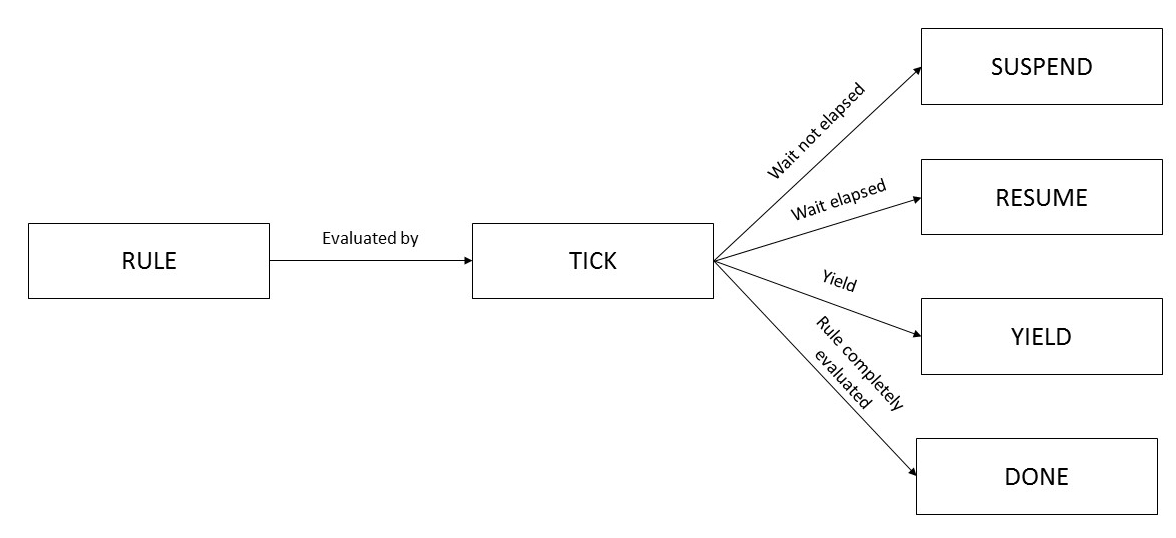
\includegraphics[width=\textwidth]{Figures/tick}
	\caption{Possible results of the \texttt{tick} function}
	\label{fig:ch_mcnv_languages_tick_result}
\end{figure}

\begin{lstlisting}
Data "rule" -> List[<<string>>] -> stmt -> stmt -> <<ImmutableDictionary<string, Value> >>  -> <<float>> : Rule
Data "Done" -> ctxt : ExecutionResult
Data "Suspend" -> stmt -> ctxt : ExecutionResult
Data "Yield" -> stmt -> List[Value] -> ctxt : ExecutionResult
Data "Resume" -> stmt -> ctxt : ExecutionResult
Data "Atomic" -> stmt -> ctxt : ExecutionResult
Func "tick" -> List[Rule] -> List[Rule] -> 
	<<ImmutableDictionary<string, Value> >> -> <<ImmutableDictionary<string, Value> >> -> <<float>> : GameState   
\end{lstlisting}

\noindent
Note that in the implementation we use a generic meta-data structure \texttt{List} instantiated with the meta-type \texttt{Rule}. A \texttt{rule} is a meta-data structure containing a list of strings representing the domain, a sequence of statements representing the rule body, a second sequence of statement representing the continuation (i.e. the statements to be evaluated in the next frame), a symbol table of local variables, and the frame time difference.

As stated above, the \texttt{tick} function stops when all the rules have been evaluated, thus when both lists of rules are empty. In this case we return the unchanged state of the program:\newpage

\begin{lstlisting}
--------------------------------------------
tick nil nil fields globals dt -> (State nil fields globals)
\end{lstlisting}

When the rule evaluation returns \texttt{Resume}, we build a rule containing the code to execute at the next frame, when the rule restarts, an empty continuation, because the current one has been moved into the body of the new rule, and the updated symbol table, since generally the rule evaluation might define some local variables. We then recursively update the remaining rules, and finally we build a new state with the rule that has to been resumed and all the other updated rules, that are stored in the state returned by the recursive call. Note that we will present the detail of \texttt{evalRule} further ahead.

\begin{lstlisting}
evalRule (rule dom body k locals delta) fields globals -> Resume cont (Context newLocals newFields newGlobals)
r := rule dom cont nop newLocals dt
tick originals rs newFields newGlobals dt -> (State updatedRules updatedFields updatedGlobals)
st := State (r::updatedRules) updatedFields updatedGlobals
------------------------------------------------------
tick (original::originals) ((rule dom body k locals delta)::rs) fields globals dt -> st
\end{lstlisting}

\noindent
For instance, consider the rule in Listing \ref{code:ch_mcnv_languages_rule_example} and assume that \texttt{dt = 1.0}.

\begin{lstlisting}[caption = Rule example with interruption, label = code:ch_mcnv_languages_rule_example]
rule X =
  wait 1.0f
  yield X + 1
\end{lstlisting}

\noindent
After evaluating the \texttt{wait} statement, the rule evaluation would return \texttt{Resume} containing the following continuation:

\begin{lstlisting}
cont = yield X + 1
\end{lstlisting}

\noindent
The new rule that will be generated is therefore

\begin{lstlisting}
rule X =
  yield X + 1
\end{lstlisting}

\noindent
In the case of \texttt{Yield} the procedure is analogous, since \texttt{yield} pauses the rule execution for one frame and thus the continuation must be used to rebuild a new rule with the continuation in its body.

\begin{lstlisting}
evalRule (rule dom body k locals delta) fields globals -> Yield cont values (Context newLocals newFields newGlobals)
r := rule dom cont nop newLocals dt
tick originals rs newFields newGlobals dt -> (State updatedRules updatedFields updatedGlobals)
st := State (r::updatedRules) updatedFields updatedGlobals
------------------------------------------------------
tick (original::originals) ((rule dom body k locals delta)::rs) fields globals dt -> st
\end{lstlisting}

For instance, let us consider again the rule

\begin{lstlisting}
rule X =
  yield X + 1
\end{lstlisting}

\noindent
Its evaluation will generate a rule with an empty body, such as

\begin{lstlisting}
rule X = nop
\end{lstlisting}

\noindent
When the rule evaluation returns \texttt{Done}, it means that the rule statements have been completely evaluated. In this case the rule must pause for one frame. It is also necessary to rebuild the body of the rule as it was before its execution started. Indeed, during the execution, the rule body is ``broken'' when evaluating the body because the executed statements are thrown away during the recursive calls. In the previous examples we have seen this process in action (see Listing \ref{code:ch_mcnv_languages_rule_example}). As we can see in the meta-language rule below, this time we build a new set of rules by placing the rule in its original state.

\begin{lstlisting}
evalRule r fields globals -> Done (Context newLocals newFields newGlobals)
tick originals rs newFields newGlobals dt -> (State updatedRules updatedFields updatedGlobals)
st := State (original::updatedRules) updatedFields updatedGlobals
---------------------------------------------
tick (original::originals) (r::rs) fields globals dt -> st
\end{lstlisting}

\noindent
Finally, when the rule evaluation returns \texttt{Suspend}, we obtain the updated state of the \texttt{wait} statement (when the timer is updated) and a continuation. In this case we rebuild a rule whose body contains the updated \texttt{wait} statement and the continuation. 

\begin{lstlisting}
evalRule (rule dom body k locals delta) fields globals -> Suspend (s;cont) (Context newLocals newFields newGlobals)
r := rule dom s cont newLocals dt
tick originals rs newFields newGlobals dt -> (State updatedRules updatedFields updatedGlobals)
st := State (r::updatedRules) updatedFields updatedGlobals
------------------------------------------------------
tick (original::originals) ((rule dom body k locals delta)::rs) fields globals dt -> st
\end{lstlisting}

\noindent
For instance, consider again the rule in Snippet \ref{code:ch_mcnv_languages_rule_example} but this time with \texttt{dt = 0.5}. The rule update this time returns \texttt{Suspend} (because the timer has not elapsed yet) with:

\begin{lstlisting}
s = wait 0.5f
cont = yield X + 1
\end{lstlisting} 

\noindent
thus the new rule will look like:

\begin{lstlisting}
rule X =
  wait 0.5f
  yield X + 1
\end{lstlisting}

\noindent
A summary of this process can be seen in Figure \ref{fig:ch_mcnv_languages_tick}.

\begin{figure}
	\centering
	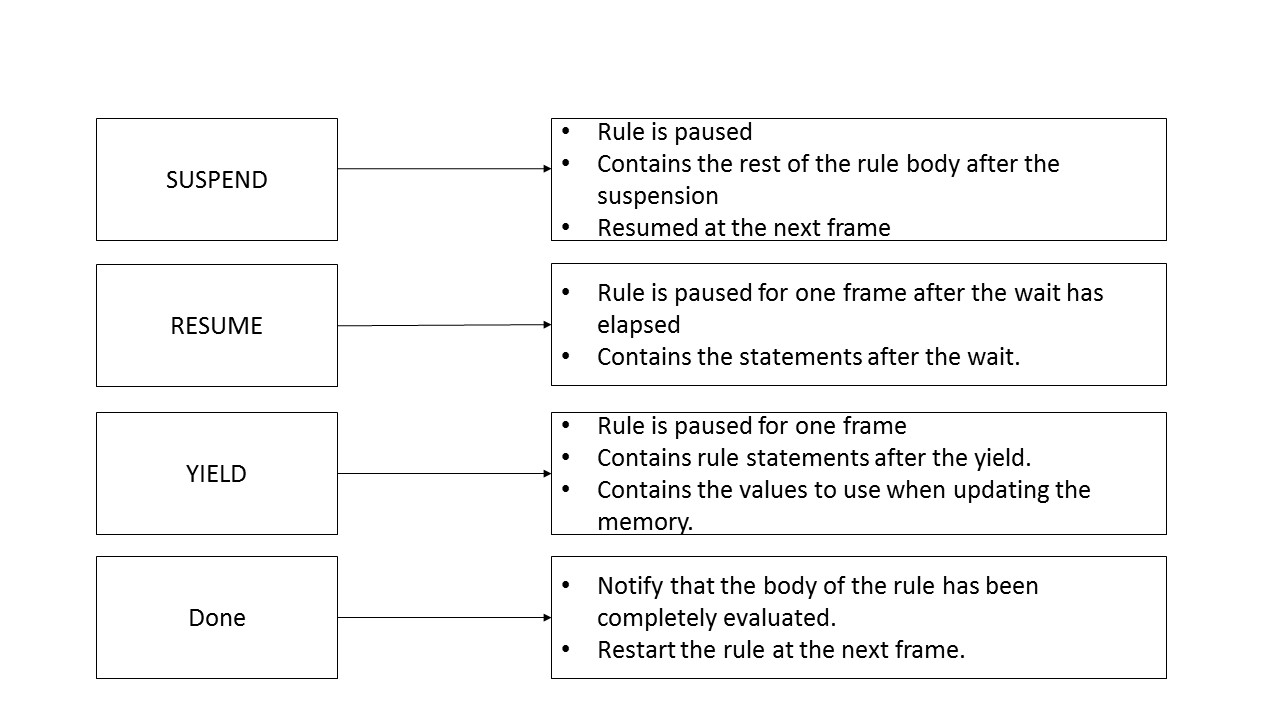
\includegraphics[width=\textwidth]{Figures/tick2}
	\caption{Cases of rule update}
	\label{fig:ch_mcnv_languages_tick}
\end{figure}

\subsection{Rule evaluation}
\label{subsec:ch_mcnv_languages_rule_evaluation}

The function \texttt{evalRule} takes as input a rule and the symbol tables for the current entity and the \texttt{world} and returns an execution result, as seen in Section \ref{subsec:ch_mcnv_languages_rule_update}.

\begin{lstlisting}
Func "evalRule" -> Rule -> <<ImmutableDictionary<string, Value> >> -> <<ImmutableDictionary<string, Value> >> : ExecutionResult
\end{lstlisting}

\noindent
Semantics rules having \texttt{evalRule} in their conclusion call in one of their premises the function \texttt{eval\tu s}. This function is able to process a sequence of statements and return a result depending on the current statement being executed. When \texttt{eval\tu s} returns \texttt{Done}, \texttt{Suspend}, or \texttt{Resume}, \texttt{evalRule} simply forwards the result to \texttt{tick} as it is. On the other hand, \texttt{eval\tu s} can also return \texttt{Yield} and an additional result called \texttt{Atomic}. This kind of result represents a statement that does not pause the rule execution. \texttt{Atomic} statements are evaluated within the current frame until an interruption statement or the end of the rule is reached.

In the case of \texttt{Yield}, the function must update the fields of the entity before returning the result to \texttt{tick}, as shown below:

\begin{lstlisting}
eval_s b k (Context locals fields globals) dt -> Yield ks values context
updateFields dom values context  -> updatedContext
-----------------------------------------
evalRule (rule dom b k locals dt) fields globals -> Yield ks values updatedContext
\end{lstlisting}

\noindent
We omit the implementation details of \texttt{updateFields} for brevity; suffice to say that this function evaluates the expressions contained in \texttt{yield} and writes their values in the symbol table.

In the case of \texttt{Atomic}, the rule must immediately be re-evaluated in the current frame. This is obtained by recursively calling \texttt{evalRule} again with the current rule whose body has been replaced by the continuation returned by \texttt{Atomic} (which is simply the remaining code in the rule body).

\begin{lstlisting}
eval_s b k (Context locals fields globals) dt -> Atomic z (Context newLocals newFields newGlobals)
evalRule (rule dom z nop newLocals dt) newFields newGlobals -> res
-----------------------------------------
evalRule (rule dom b k locals dt) fields globals  -> res
\end{lstlisting}

A schematic representation of the interaction between \texttt{tick} and\\ \texttt{evalStatement} can be seen in Figure \ref{fig:ch_mcnv_languages_rule_update}.

\begin{figure}
	\centering
	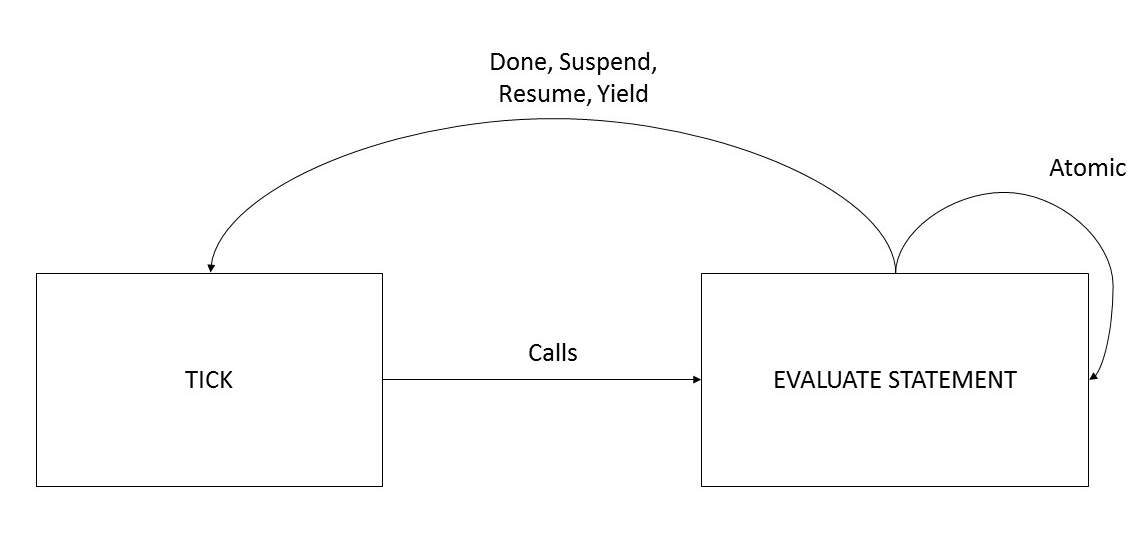
\includegraphics[width=\textwidth]{Figures/statement_evaluation}
	\caption{Rule update in Metacasanova}
	\label{fig:ch_mcnv_languages_rule_update}
\end{figure}

\subsection{Statement evaluation}
Statement evaluation is implemented through the function \texttt{eval\tu s}. This function takes as input a sequence of statements or a single statement and returns a different result depending on the statement semantics. This function takes as input the current body of the rule, its continuation and the context of the program made by the symbol tables of \texttt{world}, the current entity, and the local variables of the rule.

\begin{lstlisting}
Func "eval_s" -> stmt -> stmt -> ctxt -> <<float>> : ExecutionResult
\end{lstlisting}

\noindent
The base case of \texttt{eval\tu s} is when the body of the rule is empty and there is no continuation. This is the case when the whole rule body has been executed and thus we have to return \texttt{Done}.

\begin{lstlisting}
-------------------------------
eval_s nop nop ctxt dt -> Done ctxt
\end{lstlisting}

\noindent
When the rule body is non-empty, then we must extract the first statement in the statement sequence. We then combine the remaining body of the rule with the current continuation into a single statement sequence by using the function \texttt{addStmt}. This function has two cases: (\textit{i}) both the remaining body of the rule and the continuation are empty, or (\textit{ii}) the body of the rule is non-empty. The first case happens when we are executing the last statement in the rule body. In this case we generate an empty continuation containing \texttt{nop}. In the second case we simply combine the remaining body of the rule and the continuation into a single statement sequence.

\begin{lstlisting}
a != nop
---------------------
addStmt a b -> a;b

-------------------
addStmt nop nop -> nop
\end{lstlisting}

\noindent
Note that the case where only \texttt{b} is \texttt{nop} cannot be generated, because executing a statement will always generate a non-empty continuation, unless it is the last statement of the rule to be executed. This case is captured by \texttt{eval\tu s} (as shown above), which will return \texttt{Done}. When \texttt{Done} is forwarded as result to \texttt{tick}, the body of the rule will be regenerated by replacing it with the initial code of the rule (we reset the rule) as shown in Section \ref{subsec:ch_mcnv_languages_rule_update}.

After the new continuation has been generated, we recursively call \texttt{eval\tu s} by giving it as input the first statement in the rule body.

\begin{lstlisting}
addStmt b k -> cont
eval_s a cont ctxt dt -> res
-------------------------------
eval_s (a;b) k ctxt dt -> res
\end{lstlisting}

We now proceed to show how the semantics of the statements is implemented

\subsubsection{Interruptible statements}
Interruptible statements are statements that can pause the execution of a rule: \texttt{wait} and \texttt{yield}. As briefly pointed out before, \texttt{yield} returns as result a meta-data structure \texttt{Yield} containing the continuation of the rule to resume at the next frame, the values to write in the domain fields, and the current program context (the symbol tables). Since the arguments of \texttt{yield} can be expressions, its semantics must evaluate them one by one and return their values.

\begin{lstlisting}
-------------------------
evalYield nil ctxt -> nil

eval expr ctxt -> v
evalYield exprs ctxt -> vs
-------------------------------------------
evalYield (expr :: exprs) ctxt -> v :: vs


evalYield exprs ctxt -> values
------------------------------------------------------
eval_s (yield exprs) k ctxt dt -> Yield k values ctxt
\end{lstlisting}

\noindent
The statement \texttt{wait} in Casanova has double semantics: one waits for a timer to elapse and the other until a certain condition is met. In Metacasanova we do not have overloading, thus we are forced to use a different name to model both cases of its semantics. We use \texttt{wait} for the timed and \texttt{when} for the conditional version of the statement.

For the timed version we have two cases: (\textit{i}) the timer has elapsed and we can resume the execution of the rule at the next frame, or (\textit{ii}) the timer is still running, thus we have to suspend the rule. In the first case we return \texttt{Resume} containing the current continuation of the rule body. In the other case we have to suspend the rule, thus we return \texttt{Suspend} where the continuation contains \texttt{wait}, whose timer has been updated by removing \texttt{dt}, concatenated to the current continuation of the rule.

\begin{lstlisting}
eval expr ctxt -> ($f t)
t > dt
<<t - dt>> -> t'
----------------------------------
eval_s (wait expr) k ctxt dt -> Suspend (wait $f t');k ctxt

eval expr ctxt -> ($f t)
t <= dt
----------------------------------
eval_s (wait expr) k ctxt dt -> Resume k ctxt
\end{lstlisting}

\noindent
The implementation of \texttt{when} is analogous: if the condition is not met then we simply return \texttt{Suspend} where the continuation contains \texttt{when} concatenated with the previous continuation. Otherwise we return \texttt{Resume} containing the current continuation.

\begin{lstlisting}
eval expr ctxt -> ($b true)
---------------------------------------------
eval_s (when expr) k ctxt dt -> Atomic k ctxt

eval expr ctxt -> ($b false)
------------------------------------------
eval_s (when expr) k ctxt dt -> Suspend (when expr);k ctxt
\end{lstlisting}

\subsubsection{Control strucutres}
Casanova supports a conditional control structure (\texttt{if-then-else}), and two iterative control structures (\texttt{while-do} and \texttt{for-do}). The only difference with the usual semantics of control structures lies in \texttt{for-do}, which is like that of Python and F\# as it takes as input a variable that is used to iterate through the elements of a list.

The implementation of the control structures is similar to that of C-{}- with the difference that their body can be interrupted as well. At this purpose, the semantics rules must generate an appropriate continuation that will be handled by \texttt{tick}. The conditional control structure checks if the condition is true or false to select the appropriate code block to execute. After that it returns an \texttt{Atomic} result containing the concatenation of the selected code block with the current continuation of the rule. This is because the evaluation of the condition is an atomic process, i.e. must not pause the execution of the rule. The first statement of the selected code block will be executed immediately after.

\begin{lstlisting}
eval cond ctxt -> $b true
---------------------------------------------
eval_s (if cond then b else c) k ctxt dt -> Atomic b;k ctxt

eval cond ctxt -> $b false
---------------------------------------------
eval_s (if cond then b else c) k ctxt dt -> Atomic c;k ctxt
\end{lstlisting}

\noindent
\texttt{while-do} follows the same behaviour described in C-{}-, thus if the condition is false we simply skip the loop, otherwise we execute the body followed by the same loop. This time we must encapsulate the code built after the evaluation of the condition in an \texttt{Atomic} result, because the body must be immediately evaluated after checking the condition, as for conditionals.

\begin{lstlisting}
eval cond ctxt -> $b true
----------------------------------------------
eval_s (while cond b) k ctxt dt -> Atomic b;((while cond b);k) ctxt

eval cond ctxt -> $b false
----------------------------------------------
eval_s (while cond b) k ctxt dt -> Atomic k ctxt
\end{lstlisting}

\noindent
The semantics of \texttt{for-do} loop are quite different than what we had defined for C-{}-. The loop defines a variable that is used to iterate each element of a list. The list can be given directly or be an expression that returns a list. Thus, we have to first add to the local variables the one defined in the loop, then evaluate the expression for the list, and finally evaluate the body of the loop itself. Note that lists here are considered lists in the Casanova language and not lists of Metacasanova (thus they are values in Casanova and not meta-data structures).

\begin{lstlisting}
eval expr ctxt -> ($l nil)
------------------------------------------
eval_s (for v in expr b) k ctxt dt -> Atomic k ctxt

eval expr (Context locals e w) -> ($l (x :: xs))
locals add var x -> updatedLocals
------------------------------------------
eval_s (for ($ var) in expr b) k (Context locals e w) dt -> Atomic b;((for ($ var) in ($l xs) b);k) (Context updatedLocals e w)
\end{lstlisting}

\noindent
The base case of the evaluation is when the list is empty. In this case we simply return \texttt{Atomic} containing the current continuation because the loop can be skipped. The recursive case is when the list is non-empty: in this case we first evaluate the expression of the list, then we add the variable defined in the loop to the local variables, assigning it the value of the head of the list. We finally return an \texttt{Atomic} that contains a continuation where the body of the loop is concatenated to the loop itself and the current continuation. \texttt{Atomic} will also contain a program context where the locals now contain the new variable defined in the loop.

Note that, for simplicity, we do not have code block scoping like in C-{}-. This feature can be implemented by replacing the local symbol table with a list of tables as previously shown in Section \ref{subsec:ch_mcnv_languages_expression_semantics}.

\section{Evaluation}
\label{sec:ch_mcnv_languages_evaluation}
In this section we compare the runtime performance of a program written for C-{}- and Casanova implemented in Metacasanova with their equivalent implementation in Python. Moreover, we evaluate the length of the language definition in Metacasanova with respect to their hard-coded implementation. In total we ran one test for several executions of a program written in C-{}- against the same implementation in Python, and five tests for a program in the meta-compiled version of Casanova against the Python implementation by varying the entity number. The details of the setup are described below.

\subsection{Experimental Set-up}
We evaluated C-{}- and the meta-compiled Casanova runtime performance against an equivalent implementation of equivalent programs in Python. C-{}- was tested running a program to compute the factorial, while we implemented a program in Metacasanova where some entities patrol an area according to pre-defined checkpoints. In the case of Casanova, this language was chosen based on its use in game development: Python has been used extensively in several games such as Civlization IV \cite{CIV4} and World in Conflict \cite{WIC} because of the native support for coroutines that allow to implement a behaviour similar to that of Casanova rules. In the case of C-{}-, we still use Python because, as we discuss further ahead, the behaviour of this language is much more similar to that of a dynamic language (the name was chosen mainly because of a lack of creativity from the author than because of its similarity with C). As for the code length, we compare the length of the semantics definition of C-{}- with a hard-coded implementation, while we compare the definition of Casanova in Metacasanova with respect to its hard-coded compiler written in F\#.

For Casanova we use a program where a Casanova entity patrols a set of checkpoints. When the entity reaches the position of a checkpoint it will move to the next one. The same code has been re-implemented in Python using coroutines to simulate the interruption mechanism of rule statements that is built-in in Casanova. The code generated by the version of Casanova implemented in Metacasanova was imported in a C\# program for Monogame but tested in isolation to actually measure only the running time of the logic, which would otherwise be influenced by the rendering time and the overhead of Monogame itself. We run the Casanova program and the Python version with a variable number of entities (that will be updated) ranging from 100 to 250. For each execution we measure the time taken to update them all for each frame, and we average this time on the number of total frames. As for the code length of the language definition, we measure the length of the language specification in Metacasanova and we compare it with the relative parts of code in the hard-coded version of the compiler.

This code has also been tested by including it in a Monogame project. The program code generated with the Metacompiler updates the logic of the entities that are drawn using the Monogame framework. In this way the logic of the game is written in the meta-compiled version of Casanova and the external framework is used only for the graphical part. This has the advantage that the same code can be re-used in another game engine that is able to run .NET code (for instance Unity). A schematic representation of the integration with Monogame is shown in Figure \ref{fig:ch_mcnv_languages_monogame_integration}

\begin{figure}
	\centering
	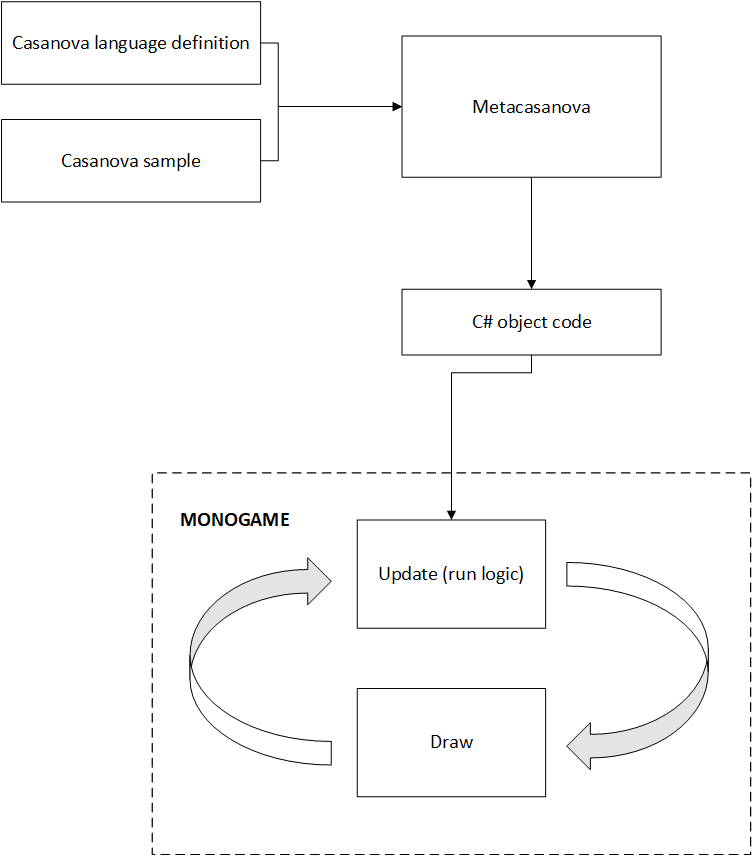
\includegraphics[width = \textwidth]{Figures/chapter_languages/monogame_integration}
	\caption{Integration of meta-compiled Casanova in Monogame}
	\label{fig:ch_mcnv_languages_monogame_integration}
\end{figure}

\subsection{Performance}
From Table \ref{tab:ch_mcnv_languages_casanova_compiler_comparison} we see that the implementation of Casanova 2.0 language in Metacasanova is almost 5 times shorter in terms of lines of code than the hard-coded implementation of the Casanova compiler written in F\#, while the C-{}- implementation is 11 times shorter (Table \ref{tab:mcnv_languages_cmm}). We believe it is worthy noticing that structures with complex behaviours, such as \textit{wait} or \textit{when}, require hundreds of lines of codes with a standard approach (the code lines to define the behaviour of the structure plus the support code to correctly generate the state machine), while in the meta-compiler we just need tens of lines of codes to implement the same behaviour. Moreover we want to point out that the previous Casanova compiler was written in a functional programming language: these languages tend to be more synthetic than imperative languages, so the difference with the same compiler implemented in languages such as C/C++ might be even greater.

The readability with respect to the hard-coded compiler code is also improved: we managed to implement the behaviour of synchronization and timing primitives almost imitating one to one the formal semantics of the language definition. In the hard-coded compiler implementation for Casanova 2.0 the semantics are lost in the code for generating finite state machines. Just for comparison, Figure \ref{fig:ch_mcnv_languages_wait_code_generation} shows the code from the Casanova hard-coded compiler to generate part of the state machine necessary to simulate the behaviour of the timed version of \texttt{wait} (the code generation of \texttt{when} has about the same size).

\begin{figure}
	\centering
	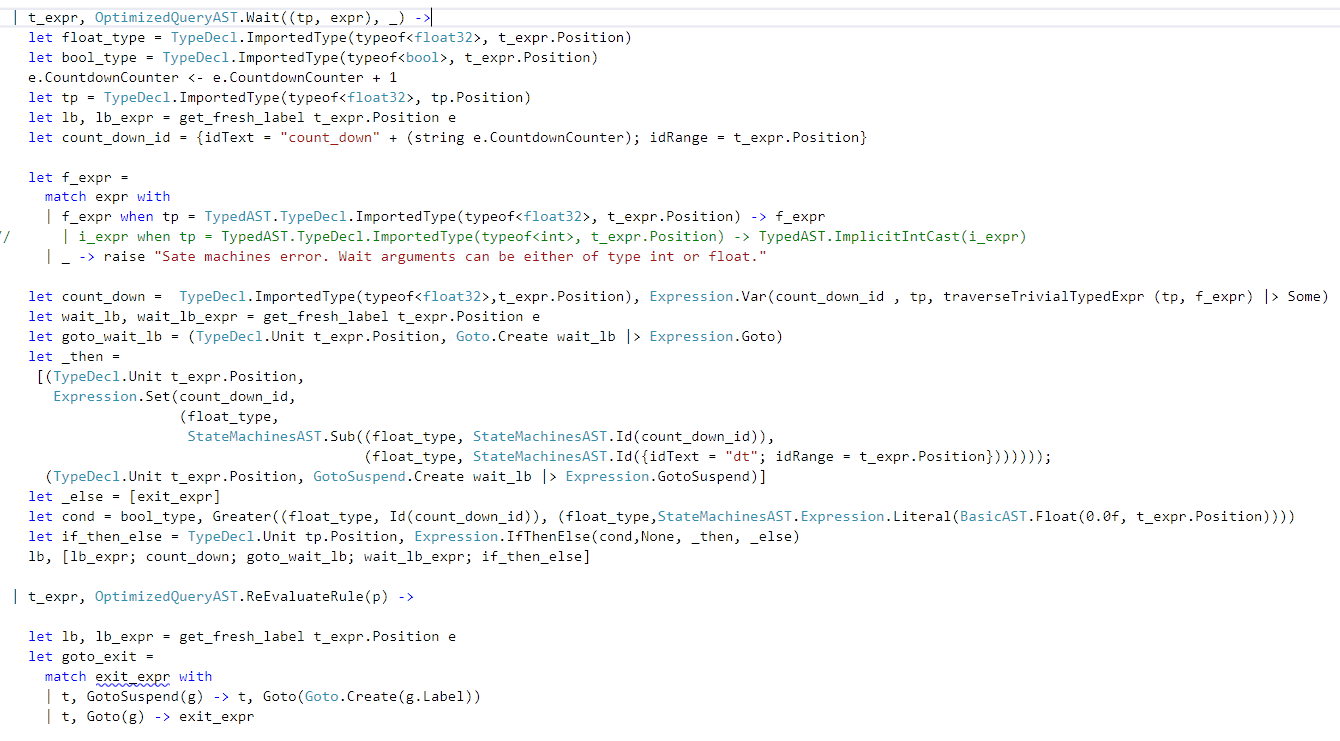
\includegraphics[angle = 90,scale= 0.6]{Figures/wait_code_casanova_compiler}
	\caption{Code generation of \texttt{wait} in the Casanova compiler}
	\label{fig:ch_mcnv_languages_wait_code_generation}
\end{figure}

The performance results are shown in Table \ref{tab:ch_mcnv_casanova_evaluation}. We see that the generated code has performance on the same order of Python, although 3 times slower. This gap is accentuated in the case of C-{}-, which is 50 times slower than Python, because in the case of a simple imperative program, where the use of virtual tables for polymorphic types (as coroutines) is limited, the speed of Python greatly increases.

\begin{table}
	\centering
	\begin{tabular}{|c|c|c|}
		\hline
		\multicolumn{3}{|c|}{\textbf{Meta-compiled Casanova}} \\
		\hline
		Entity \# & Average update time (s) & Frame rate \\
		\hline
		100 & 0.00349 & 286.53 \\
		\hline
		250 & 0.00911 & 109.77 \\
		\hline
		500 & 0.01716 & 58.275 \\
		\hline
		750 & 0.02597 & 38.506 \\
		\hline
		1000 & 0.03527 & 28.353 \\
		\hline
		\multicolumn{3}{|c|}{\textbf{Python}} \\
		\hline
		Entity \# & Average update time (s) & Frame rate \\
		\hline
		100 & 0.00132 & 756.37 \\
		\hline
		250 & 0.00342 & 292.05 \\
		\hline
		500 & 0.00678 & 147.54 \\
		\hline
		750 & 0.01087 & 91.988 \\
		\hline
		1000 & 0.01408 & 71.002 \\
		\hline
	\end{tabular}
	\caption{Patrol sample evaluation}
	\label{tab:ch_mcnv_casanova_evaluation}
\end{table}

\begin{table}
	\centering
	\begin{tabular}{|c|c|}
		\hline
		\multicolumn{2}{|c|}{\textbf{Meta-compiled Casanova}} \\
		\hline
		Module & Code lines \\
		\hline
		Data structures and function definitions & 40 \\
		\hline
		Query Evaluation & 16 \\
		\hline
		While loop & 4 \\
		\hline
		For loop & 5 \\
		\hline
		If-then-else & 4 \\
		\hline
		When & 4 \\
		\hline
		Wait & 6 \\
		\hline
		Yield & 10 \\
		\hline
		Additional rules for Casanova program evaluation & 40 \\
		\hline
		Additional rules for basic expression evaluation & 201 \\
		\hline
		\multicolumn{2}{|l|}{\textbf{Total: } 300} \\
		\hline
		\multicolumn{2}{|c|}{\textbf{Casanova 2.0 compiler}} \\
		\hline
		Module & Code lines \\
		\hline
		While loop & 10 \\
		\hline
		For-loop and query evaluation & 44 \\
		\hline
		If-Then-Else & 15 \\
		\hline
		When & 11 \\
		\hline
		Wait & 24 \\
		\hline
		Yield & 29 \\
		\hline
		Additional structures for rule evaluation & 63 \\
		\hline
		Structures for state machine generations & 754 \\
		\hline
		Code generation & 530 \\
		\hline
		\multicolumn{2}{|l|}{\textbf{Total: } 1480} \\
		\hline			
	\end{tabular}	
	\caption{meta-compiler vs standard compiler}
	\label{tab:ch_mcnv_languages_casanova_compiler_comparison}
\end{table}

\begin{table}
	\centering
	\begin{tabular}{|c|c|c|}
		\hline
		\textbf{Statement} & \textbf{Metacasanova} & \textbf{C\#}\\
		\hline
		\texttt{if-then-else} & 4 & 103 \\
		\hline
		\texttt{while} & 7 & 73 \\
		\hline
		\texttt{For} & 11 & 81\\
		\hline
	\end{tabular}
	
	\vspace{0.15cm}
	\begin{tabular}{|c|c|}
		\hline
		\textbf{C-{}-} & \textbf{Python} \\
		\hline
		1.26ms & $2.36 \cdot 10^{-2}$ms \\
		\hline
	\end{tabular}
	\caption{Code length implementation of C-{}- and run-time performance}
	\label{tab:mcnv_languages_cmm}
\end{table}

\subsection{Discussion}
\label{subsec:code_generation_discussion}
Even though the size of the code required to implement the language has been drastically reduced (almost 1/5 shorter), performance dropped dramatically. The problem lies in the fact that, in order to implement a memory model, in the current version of Casanova we must rely on dynamic access to a symbol table at runtime. Indeed, when we define a new variable or read its value, the semantics contain a rule defining the insertion or the lookup of the variable. Metacasanova generates the code able to run those rules, but the memory operations are thus executed at runtime as dictionary operations.

In order to encode a symbol table in the meta-compiler in the current implementation (used for example to store the variables defined in the local scope of a control structure or to model a class/record data structure), we are left with two options: (\textit{i}) define a custom data structure made of a list of pairs, containing the field/variable name as a string and its value, in the following way

\begin{lstlisting}
Data "table" -> List[Tuple[string, Value]] : SymbolTable
\end{lstlisting}

\noindent
or (\textit{ii}) use a dictionary data structure coming from .NET, such as\\ \texttt{ImmutableDictionary} \footnote{For a motivation about the choice of the dictionary implementation we point the reader to Section \ref{sec:ch_functors_evaluation}}, which was the implementation choice for Casanova. In both cases, the behaviour of the language implemented in Metacasanova will be that of a dynamic language, because whenever the value of a variable or class field must be read, the evaluation rule must look up the symbol table at run time to retrieve the value.

The same applies to type checking: in Section \ref{subsec:ch_mcnv_languages_type_checking} we showed the type rules that check the types of a C-{}- program. In statically-typed languages, type checking is usually performed at compile time and not at runtime. However, in this case Metacasanova will again generate the code to run the type rules, but the actual execution is performed when the program is run, thus the behaviour of C-{}- is more similar to that of a dynamic language rather than a static language (and its performance as well).

This issue is caused by the fact that, in the current state of Metacasanova, the meta-type system is unaware of the type system of the language that is being implemented in the meta-compiler. This means that, as it is, the meta-language is unable to define a statically-typed language. This is not a problem limited to Metacasanova but to all meta-compilers having a meta-type system that does not allow embedding of the object language type system. 

The same applies for the lookup: the access to symbol tables needs not to be dynamic because the symbol table does not grow when the program runs, thus the access to a specific variable could be directly inlined in the code. For example, if we want to access variable \texttt{x}, which is the third entry of the symbol table, we will always perform the same lookup. Thus, this lookup could be simply inlined as an access to the third element of the symbol table. An analogous situation happens for Casanova entities: their structure does not change at runtime, so if we access, for instance, a field of an entity and that is the third one, then we always perform a lookup on the third element of the symbol table, and this can be inlined directly as well.

\section{Summary}
In this chapter we showed two examples of how to use Metacasanova to implement programming languages. We started by showing how to implement a small imperative language called C-{}-. We showed an implementation of its semantics and then of its type system. Later we re-implemented the Casanova language, a DSL for game development. We showed how to implement the semantics of interruptible code, which in Casanova had been implemented with state machines, by using continuation-passing style. Metacasanova implementation of Casanova results to be 5 times shorter than that of the hard-coded compiler for Casanova written in F\#. In the case of C-{}- the gap in terms of lines of code is even larger, being the code for its semantics 11 times shorter than a hard-coded implementation. However, the code performance drops dramatically: testing the meta-compiled version of Casanova against Python results in its code being 3 times slower (although on the same order of magnitude), while the C-{}- code is even 50 times slower. The cause of this is that, even thought these languages could be statically-typed, the rule evaluation performs the lookup of variables and types at runtime. This cannot be changed with the Metacasanova language abstractions presented so far because the meta-type system of Metacasanova is unaware of the types of the embedded language (i.e. the language that is being implemented in Metacasanova). In the next chapter we will show a language extension for Metacasanova that relies on \textit{Functors} to embed the type system of languages implemented in Metacasanova in its type system, and to inline the access to variables at compile time.